\documentclass[aspectratio=169,11pt]{beamer}

% ───────────────────────────────────────────────────────────────────────── %
% Tema visual: cremoso + titulo serif navy, mismo que avance_4.              %
% ───────────────────────────────────────────────────────────────────────── %
\usepackage[utf8]{inputenc}
\usepackage[T1]{fontenc}
\usepackage[spanish,es-tabla]{babel}
\usepackage{lmodern}
\usepackage{amsmath,amssymb}
\usepackage{graphicx}
\usepackage{booktabs}
\usepackage{array}
\usepackage{xcolor}
\usepackage{colortbl}
\usepackage{tikz}
\usepackage{microtype}
\usepackage{pifont}

% Paleta
\definecolor{cream}{HTML}{F2EEE3}
\definecolor{navy}{HTML}{2F3E4E}
\definecolor{accentA}{HTML}{7E57C2}
\definecolor{accentB}{HTML}{EF6C00}
\definecolor{accentC}{HTML}{2E7D32}
\definecolor{accentD}{HTML}{C62828}
\definecolor{rule}{HTML}{B5AFA1}

\setbeamercolor{background canvas}{bg=cream}
\setbeamercolor{normal text}{fg=navy}
\setbeamercolor{frametitle}{fg=navy,bg=cream}
\setbeamercolor{title}{fg=navy}
\setbeamercolor{author}{fg=navy}
\setbeamercolor{structure}{fg=accentC}
\setbeamercolor{itemize item}{fg=accentC}
\setbeamercolor{itemize subitem}{fg=accentB}

\setbeamerfont{frametitle}{family=\rmfamily,series=\bfseries,size=\Large}
\setbeamerfont{title}{family=\rmfamily,series=\bfseries,size=\huge}
\setbeamerfont{subtitle}{family=\rmfamily,size=\large}

\setbeamertemplate{navigation symbols}{}
\setbeamertemplate{frametitle}{%
  \vspace{0.6em}%
  \begin{center}
    \usebeamerfont{frametitle}\usebeamercolor[fg]{frametitle}\insertframetitle
  \end{center}%
  \vspace{-0.4em}%
  {\color{rule}\hrule height 0.6pt}%
  \vspace{0.4em}%
}
\setbeamertemplate{footline}{%
  \hfill\usebeamercolor[fg]{normal text}\small\insertframenumber\hspace{1em}\vspace{0.4em}%
}

% ───────────────────────────────────────────────────────────────────────── %
\title{Sistema de Recomendaci\'on H\'ibrido\\para Pueblos M\'agicos}
\subtitle{An\'alisis de Aspectos\\
\vspace{0.4em}\textit{Seminario de Tesis}}
\author{Gustavo Hern\'andez Angeles}
\date{}

\begin{document}

% ───────────────────────────── Portada ─────────────────────────────────── %
\begin{frame}[plain]
	\vspace{1.5em}
	\begin{center}
		{\usebeamerfont{title}\color{navy}Sistema de Recomendaci\'on H\'ibrido\\para Pueblos M\'agicos}\\[0.6em]
		{\usebeamerfont{subtitle}\color{navy}An\'alisis de Sentimiento Basado en Aspectos}\\[0.3em]
		{\color{rule}\rule{0.5\linewidth}{0.4pt}}\\[0.4em]
		{\large\itshape Seminario de Tesis}
	\end{center}
	\vspace{1.2em}
	\begin{flushleft}
		\textbf{Autor:} Gustavo Hern\'andez Angeles\\
		\textbf{Asesor:} Dr.\ Norberto Alejandro Hern\'andez Leandro\\[0.3em]
		\textbf{Comit\'e de Seguimiento:}\\
		\quad$\bullet$ Dr.\ Alejandro Rosales P\'erez\\
		\quad$\bullet$ Dr.\ Miguel \'Angel \'Alvarez Carmona\\[0.5em]
	\end{flushleft}
\end{frame}

% ───────────────────────────── Objetivos ───────────────────────────────── %
\begin{frame}{Objetivos}
	\small
	\textbf{Objetivo General.}\;
	Elaborar un sistema de recomendaci\'on h\'ibrido (SRH) para Pueblos M\'agicos de M\'exico que integre ABSA, compuesto por modelos colaborativos y basados en contenido.

	\vspace{0.6em}
	\textbf{Objetivos espec\'ificos:}
	\begin{columns}[T]
		\begin{column}{0.5\linewidth}
			\begin{enumerate}\setlength\itemsep{3pt}
				\item[\color{accentC}\ding{51}] Preparar el corpus de trabajo a partir del \textit{dataset} REST-MEX 2025.
				\item[\color{accentC}\ding{51}] Pipeline de ABSA con Zero-Shot y Sentiment Classification.
				\item[\color{accentC}\ding{51}] Derivar las matrices estructurales del sistema (relaci\'on usuarios, \'items, aspectos).
			\end{enumerate}
		\end{column}
		\begin{column}{0.5\linewidth}
			\begin{enumerate}\setlength\itemsep{3pt}
				\item[\color{accentC}\ding{51}] Implementaci\'on de los modelos colaborativos y basados en contenido.
				\item[\color{accentC}\ding{51}] Implementar la fusi\'on de componentes y evaluar el SRH.
				\item[$\square$] Análisis de resultados del modelo.
			\end{enumerate}
		\end{column}
	\end{columns}

	\vspace{0.6em}
	\centering
	{\color{rule}\rule{0.4\linewidth}{0.4pt}}\\[0.3em]
	\textit{Avance actual:} \textbf{5/6} objetivos espec\'ificos completados.
\end{frame}

% ───────────────────────────── Recapitulando ───────────────────────────── %
\begin{frame}{Recapitulando...}
	\small
	Desde el \'ultimo avance: pipeline ABSA, matrices estructurales $A,X,Y,R$, y baseline de cuatro modelos con fusi\'on convexa.
	\vspace{0.6em}
	\begin{columns}[T]
		\begin{column}{0.48\linewidth}
			\textbf{Recordatorio - matrices de perfil:}
			\[
				X_{u,j}=1+(N-1)\!\left(\frac{2}{1+e^{-t_{uj}}}-1\right)
			\]
			\[
				Y_{p,j}=1+\frac{N-1}{1+e^{-k_{pj}\cdot \bar{s}_{pj}}}
			\]
			$X$: importancia usuario-aspecto.\\
			$Y$: calidad pueblo-aspecto.
		\end{column}
		\begin{column}{0.48\linewidth}
			\textbf{En este avance:}
			\begin{itemize}
				\item \textbf{Ablaci\'on $X/Y$}: explica el efecto del $\log$ y de la $T$.
				\item \textbf{Replanteamiento del h\'ibrido}: pasamos de 4 modelos a un h\'ibrido de \emph{dos} basados en aspectos.
				\item \textbf{Grid-search} sobre un \'unico $\alpha \in [0,1]$.
			\end{itemize}
		\end{column}
	\end{columns}
\end{frame}

% ─────────── Ablacion 1/3: modificaciones a Zhang et al. ──────────────── %
\begin{frame}{Ablaci\'on de $X$ y $Y$\;|\;modificaciones a Zhang et al.\ (2014)}
	\small
	Las matrices $X$ y $Y$ devuelven valores en el mismo rango que la calificaci\'on
	de usuarios, $[1, N{=}5]$, v\'ia sigmoides. Sobre la formulaci\'on original
	de Zhang et al.\ (2014) acumulamos \emph{dos} modificaciones:

	\vspace{0.6em}
	\begin{columns}[T]
		\begin{column}{0.5\linewidth}
			\textbf{(1) $\log(1+n)$ en $Y$.}
			\[
				Y_{p,j}\;\propto\;\sigma\!\left(\log(1+n_{pj})\cdot \bar{s}_{pj}\right)
			\]
			Amortigua el efecto del \textbf{volumen} de rese\~nas
			$n_{pj}$ del aspecto $j$ en el pueblo $p$: pueblos con cientos de
			rese\~nas no opacan a los menos rese\~nados.
		\end{column}
		\begin{column}{0.5\linewidth}
			\textbf{(2) Escalamiento $T$.}
			\[
				X_{u,j}\;\propto\;\sigma\!\left(t_{uj}/T_x\right),\quad
				Y_{p,j}\;\propto\;\sigma\!\left(\cdot/T_y\right)
			\]
			$T=$ mediana de los argumentos del sigmoide. Sin $T$, el sigmoide
			\textbf{satura} casi todas las celdas en $\approx 5$ y se pierde la
			discriminaci\'on entre usuarios/pueblos.
		\end{column}
	\end{columns}

	\vspace{0.8em}
	\centering
	\textit{¿Cu\'al de las dos modificaciones es la que realmente sostiene el desempe\~no?}
\end{frame}

% ─────────── Ablacion 2/3: diseno del estudio ──────────────────────────── %
\begin{frame}{Ablaci\'on de $X$ y $Y$\;|\;dise\~no del estudio}
	\small
	Dise\~no factorial: cruzamos las dos modificaciones (presente/ausente) sobre
	los modelos sensibles a $X$ y/o $Y$: \texttt{CBQuality} (usa $X,Y$) y
	\texttt{CFAttention} (usa s\'olo $X$).

	\vspace{0.4em}
	\begin{columns}[T]
		\begin{column}{0.55\linewidth}
			\centering
			\scriptsize
			\renewcommand{\arraystretch}{1.15}
			\setlength{\tabcolsep}{4pt}
			\begin{tabular}{c l l}
				\toprule
				\textbf{Var.} & \textbf{$X$} & \textbf{$Y$}  \\
				\midrule
				A             & $+T$         & $\log(1+n)+T$ \\
				B             & Zhang puro   & Zhang puro    \\
				C             & Zhang puro   & $+T$          \\
				D             & $+T$         & $+T$          \\
				\bottomrule
			\end{tabular}
		\end{column}
		\begin{column}{0.43\linewidth}
			\textbf{Comparaciones:}
			\begin{itemize}\setlength\itemsep{2pt}
				\item $\mathbf{A}\leftrightarrow\mathbf{D}$: aisla el efecto del $\log(1+n)$ en $Y$ (misma $X$).
				\item $\mathbf{B}\leftrightarrow\mathbf{C}$: aisla el efecto de $T$ en $Y$ (misma $X$).
				\item $\mathbf{C}\leftrightarrow\mathbf{D}$: aisla el efecto de $T$ en $X$ (misma $Y$).
			\end{itemize}
			\vspace{0.4em}
			\textbf{M\'etricas:} NDCG@10, Cov@10, Hit@10.
		\end{column}
	\end{columns}

	\vspace{0.5em}
	\textbf{Sanity check.}\;\texttt{CFAttention} s\'olo usa $X$: variantes con
	la misma $X$ deben producir m\'etricas id\'enticas (esperamos $\text{A}{=}\text{D}$
	y $\text{B}{=}\text{C}$).
\end{frame}

% ─────────── Ablacion 3/3: hallazgos y decision ────────────────────────── %
\begin{frame}{Ablaci\'on de $X$ y $Y$\;|\;hallazgos y decisi\'on}
	\small
	\centering
	\renewcommand{\arraystretch}{1.08}
	\setlength{\tabcolsep}{8pt}
	\begin{tabular}{c c c c}
		\toprule
		\textbf{Var.} & NDCG@10         & Cov@10          & Hit@10          \\
		\midrule
		A             & 0.3358          & 0.6458          & 0.5714          \\
		B             & 0.2778          & 0.6458          & 0.5988          \\
		C             & \textbf{0.3666} & 0.7083          & \textbf{0.6285} \\
		\rowcolor{cream!50}
		D             & 0.3658          & \textbf{0.7292} & 0.6269          \\
		\bottomrule
	\end{tabular}

	\vspace{0.7em}
	\textbf{Hallazgos:}
	\begin{itemize}\setlength\itemsep{3pt}
		\item En $\mathbf{B}$, $Y$ \emph{satura}: $97.9\%$ de celdas $>4.5$ $\Rightarrow$ NDCG cae a $0.2778$.
		\item El escalamiento $T$ (C, D) \textbf{recupera la discriminaci\'on} entre pueblos: $+9$ puntos de NDCG y $+6$ de Cov respecto a B.
		\item El $\log(1+n)$ resultaba \textbf{redundante} (y sub-\'optimo) cuando ya hay $T$: A $<$ D pese a llevar ambas modificaciones.
	\end{itemize}

	\vspace{0.4em}
	\textbf{Decisi\'on:} se adopta la variante \textbf{D} como construcci\'on can\'on; incluimos escalamiento en ambas matrices, descartamos logaritmo.
	C y D son indistinguibles en ranking; D gana en cobertura.
\end{frame}

% ─────────────────────── Replanteamiento ───────────────────────────────── %
\begin{frame}{Replanteamiento del h\'ibrido}
	\small
	\textbf{Antes:} cuatro modelos en combinaci\'on convexa,
	$\hat y_{u,p}(\mathbf{w}) = \sum_{m=1}^{4} w_m \,\hat y^{(m)}_{u,p}$, con $\mathbf{w}\in\Delta^{3}$.

	\vspace{0.4em}
	\textbf{Hallazgos de la evaluaci\'on previa:}
	\begin{itemize}\setlength\itemsep{2pt}
		\item {\tt CBQuality} domina las m\'etricas de \textbf{ranking} (NDCG, MRR, Hit).
		\item {\tt CFAttention} domina la \textbf{cobertura} del cat\'alogo.
	\end{itemize}

	\vspace{0.5em}
	\textbf{Propuesta:} h\'ibrido de \emph{dos} modelos, ambos consumiendo se\~nales ABSA:
	\[
		\boxed{\;\hat y_{u,p}(\alpha) \;=\; \alpha\,\hat y^{\mathtt{CFAttention}}_{u,p} \;+\; (1-\alpha)\,\hat y^{\mathtt{CBQuality}}_{u,p}\;}
	\]
	El espacio de b\'usqueda se reduce a 1D $\Rightarrow$ basta un \textbf{grid-search} en $\alpha$, sin PSO/DE/BO.
\end{frame}

% ─────────────────────── Formulacion ──────────────────────────────────── %
\begin{frame}{Formulaci\'on de la b\'usqueda en $\alpha$}
	\small
	Sea $\hat y^{(m)}_{u,p}$ el score del modelo $m$. Definimos
	\[
		\hat y_{u,p}(\alpha) \;=\; \alpha\,\hat y^{\mathtt{CFAttention}}_{u,p} \;+\; (1-\alpha)\,\hat y^{\mathtt{CBQuality}}_{u,p},
		\qquad \alpha \in [0,1].
	\]
	Funci\'on objetivo: agregaci\'on lineal de ranking y diversidad,
	\[
		f(\alpha)\;=\;\beta\,\mathrm{NDCG@K}(\alpha)\;+\;(1-\beta)\,\mathrm{Cov@K}(\alpha),
		\qquad
		\alpha^{\!*} \in \arg\max_{\alpha\in[0,1]} f(\alpha).
	\]

	\vspace{0.2em}
	\textbf{Implementaci\'on barata:} {\tt CFAttention} y {\tt CBQuality} se ajustan \emph{una sola vez} y se precomputan los scores. Cada $\alpha$ del espacio de búsqueda s\'olo re-pondera los scores; no hay re-entrenamientos.
\end{frame}

% ────────────── Resultados cuantitativos: dos paneles ─────────────────── %
\begin{frame}{Resultados\;|\;m\'etricas vs.\ $\alpha$}
	\centering
	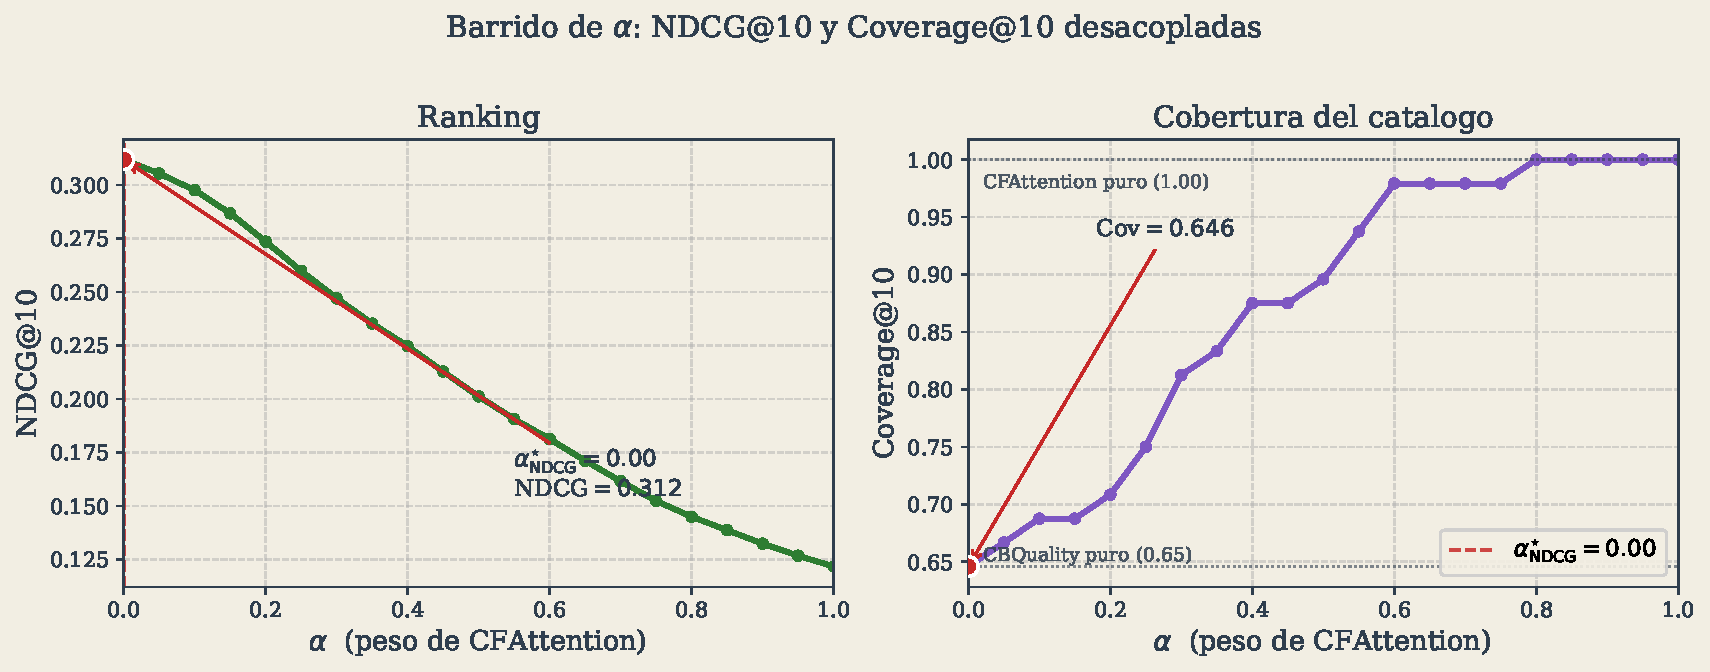
\includegraphics[width=0.88\linewidth]{figures/alpha_metrics.pdf}

	\vspace{-0.2em}
	\scriptsize
	\begin{itemize}\setlength\itemsep{1pt}
		\item \textbf{NDCG@10} es decreciente en $\alpha$: el ranking proviene de {\tt CBQuality}.
		\item \textbf{Cov@10} crece con $\alpha$ y satura en $1.0$ alrededor de $\alpha\!\approx\!0.8$: la diversidad proviene de {\tt CFAttention}.
		\item No existe un \'unico $\alpha^{*}$: la elecci\'on depende de $\beta$ (prioridad ranking vs.\ cobertura).
	\end{itemize}
\end{frame}

% ─────────────── Resultados cualitativos: tabla por alpha ──────────────── %
\begin{frame}{Resultados\;|\;c\'omo cambian las recomendaciones con $\alpha$}
	\small
	Usuario \texttt{Viajand\'isimo} — 8 pueblos en \emph{train}, 5 en \emph{test}\\
	\textit{Ground truth:} \{Isla\_Mujeres, Mazamitla, Teotihuacan, Tepoztlan, Tulum\}

	\vspace{0.5em}
	\centering
	\renewcommand{\arraystretch}{1.08}
	\setlength{\tabcolsep}{6pt}
	\begin{tabular}{c l l l}
		\toprule
		\textbf{Rank}                                         &
		\textbf{$\alpha=0.0$\;{\scriptsize(100\% CBQuality)}} &
		\textbf{$\alpha=0.5$\;{\scriptsize(mezcla)}}          &
		\textbf{$\alpha=1.0$\;{\scriptsize(100\% CFAttention)}}                                                                                                                               \\
		\midrule
		1                                                     & {\color{accentC}Tulum}\,\ding{51}         & Bacalar                                 & {\color{accentC}Teotihuacan}\,\ding{51} \\
		2                                                     & Bacalar                                   & Orizaba                                 & Xilitla                                 \\
		3                                                     & Orizaba                                   & {\color{accentC}Teotihuacan}\,\ding{51} & Orizaba                                 \\
		4                                                     & {\color{accentC}Isla\_Mujeres}\,\ding{51} & {\color{accentC}Tulum}\,\ding{51}       & Bacalar                                 \\
		5                                                     & Valladolid                                & Xilitla                                 & Metepec                                 \\
		\midrule
		\textit{Hits}                                         & 2 / 5                                     & 2 / 5                                   & 1 / 5                                   \\
		\textit{Rango score}                                  & $[4.13, 4.32]$                            & $[4.49, 4.59]$                          & $[4.87, 4.99]$                          \\
		\bottomrule
	\end{tabular}

	\vspace{0.3em}
	\scriptsize
	\begin{itemize}\setlength\itemsep{0pt}
		\item $\alpha\!=\!0$: dominan destinos de playa caribe\~na (cluster que el usuario ya frecuenta).
		\item $\alpha\!=\!0.5$: entra \texttt{Teotihuacan} (nuevo perfil, sigue acertando 2 hits).
		\item $\alpha\!=\!1$: la lista se reorienta hacia destinos m\'as ex\'oticos (\texttt{Xilitla}, \texttt{Metepec}) \!$\Rightarrow$ mayor cobertura, menor ranking.
	\end{itemize}
\end{frame}

% ─────────────────────── Cierre + proximos pasos ──────────────────────── %
\begin{frame}{Cierre y pr\'oximos pasos}
	\small
	\textbf{Lo que cerramos en este avance:}
	\begin{itemize}\setlength\itemsep{2pt}
		\item Estudio de ablaci\'on de $X/Y$: $T$ es la pieza clave; $\log(1+n)$ se elimina.
		\item Reformulaci\'on del h\'ibrido de 4 a 2 modelos (ambos ABSA-driven), grid-search 1D en $\alpha$.
		\item Caracterizaci\'on completa del \emph{trade-off} NDCG vs Cobertura como funci\'on de $\alpha$.
	\end{itemize}

	\vspace{0.6em}
	\textbf{Pr\'oximos pasos:}
	\begin{enumerate}\setlength\itemsep{2pt}
		\item Fijar $\alpha^{*}$ por criterio multi-objetivo (Pareto) o por $\beta$ acordado con el comit\'e.
		\item Cerrar redacci\'on del Cap\'itulo 4 (resultados) e iniciar correcciones para defensa.
	\end{enumerate}

	\vspace{0.6em}
	\centering
	{\color{rule}\rule{0.5\linewidth}{0.4pt}}\\[0.4em]
	\textit{Objetivos espec\'ificos del proyecto:} \textbf{5/6 completados}.\\
	\textit{Resta:} fijar $\alpha^{*}$ (Obj.\ 5) y evaluaci\'on final del SRH (Obj.\ 6).
\end{frame}

% ─────────────────────── Gracias ───────────────────────────────────────── %
\begin{frame}[plain]
	\vfill
	\begin{center}
		{\fontsize{60}{72}\selectfont\bfseries\rmfamily\color{navy}GRACIAS}
	\end{center}
	\vfill
\end{frame}

\end{document}
